\baitracnghiem{abc:b01}{%
Đường cong trong hình bên là đồ thị của một hàm số trong 
\begin{window}[0,r,{\hspace*{1cm}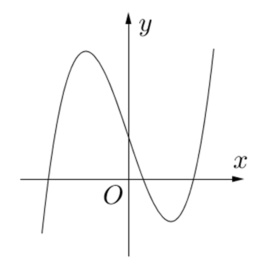
\includegraphics[scale=0.6]{toan01}\hspace*{1cm}},{\label{fig:b01}}]
bốn hàm số được liệt kê ở bốn phương án $A, B, C, D$ dưới
đây.  Hỏi hàm số đó là hàm số nào ?
\end{window}
}{
\datcot[4]
\bonpa
{\sai{$y=-x^2+x-1$.}}
{\sai{$y=-x^3+3x+1$.}}
{\dung{$y=x^3-3x+1$.}}
{\sai {$y=x^4-x^2+1$.}}
\loigiai{ 
Dựa vào đồ thị hàm số ta loại đi 2 đáp án A và C.\\
Dựa vào đồ thị hàm số ta suy ra bảng biến thiên của hàm số có dạng\\
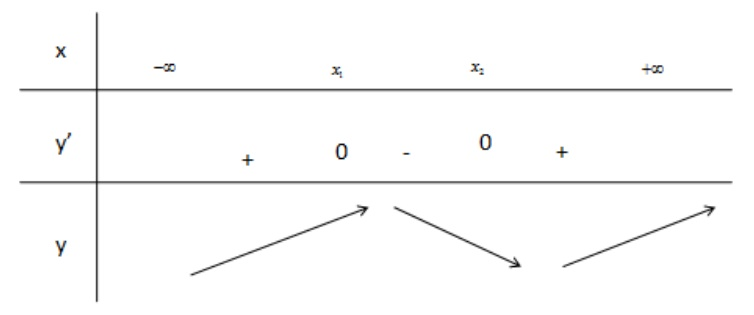
\includegraphics[scale=0.5]{gtoan01}\\
Như vậy ta thấy $y’ = 0$ có 2 nghiệm phân
 biệt và $y’$ trái dấu với hệ số của a nên hệ số $a > 0$
}
}

\baitracnghiem{abc:b02}{%
Cho hàm số $y=f(x)$ có  $\lim\limits_{x\rightarrow +\infty}f(x)=1$ và   $\lim\limits_{x\rightarrow -\infty}f(x)=-1$. Khẳng định nào sau
đây là khẳng định đúng ?
}{
\datcot[4]
\bonpa
{\sai{Đồ thị hàm số đã cho không có tiệm cận ngang.}}
{\sai{Đồ thị hàm số đã cho có đúng một tiệm cận ngang.}}
{\dung{Đồ thị hàm số đã cho có hai tiệm cận ngang là các đường thẳng  $y=1$ và  $y=-1$.}}
{\sai{Đồ thị hàm số đã cho có hai tiệm cận ngang là các đường thẳng $x=1$ và  $x=-1$.}}
\loigiai{
Vì  $\lim\limits_{x\rightarrow\infty} f(x)=1$ nên hàm số có tiệm cận ngang $y = 1$\\
Vì  $\lim\limits_{x\rightarrow-\infty} f(x)=1$ nên hàm số có tiệm cận ngang $y =-1$\\
Vậy hàm số có 2 tiệm cận ngang.
}
}

\baitracnghiem{t2017:b06}{%
Tìm giá trị nhỏ nhất của hàm số $y=\dfrac{x^2+3}{x-1}$ trên đoạn $[2;4]$.
}{
\datcot
\bonpa
{\dung{$\min_{[2;4]} y=6$.}}
{\sai{$\min_{[2;4]} y=-2$.}}
{\sai{$\min_{[2;4]} y=-3$.}}
{\sai {$\min_{[2;4]} y=\dfrac{19}{3}$.}}
\loigiai{
\begin{align*}
y&=\dfrac{x^2+3}{x-1}.\\
y'&=\dfrac{2x(x-1)-x^2-3}{(x-1)^2}=\dfrac{x^2-2x-3}{(x-1)^2}.\\
y'&=0\Leftrightarrow\left[\begin{matrix}
x=-1\quad \mbox{ loại }\\ 
x=3\quad \mbox{ thỏa mãn }\\ 
\end{matrix}\right..
\end{align*}
Có $y(2)=7; y(3)=6; y(4)=\dfrac{19}{3} \Rightarrow \min\limits_{[2;4]} y=6$.
}
}


